\documentclass[11pt, a4paper]{article}
\usepackage{multirow}
%\usepackage{minted}
\usepackage[slantfont,boldfont]{xeCJK}
\setCJKmainfont{SimSun}
\usepackage{indentfirst}
\usepackage{float}
\setlength{\parindent}{2em}
\setCJKmonofont{SimHei}
\input zhwinfonts
\renewcommand\figurename{图}
\renewcommand\tablename{表}
\renewcommand\contentsname{目录}

\begin{document}

\title{\bf 论文\\《Memory Errors in Modern Systems\\ The Good The Bad, and The Ugly》\\阅读评审报告}
\author{计算机科学与技术学院\\$\ast\ast\ast$\\115$\ast\ast\ast\ast\ast\ast\ast$}
\date{2017年5月14日}
\maketitle
\tableofcontents

\section{文章概览}

\subsection{背景}

内存系统中的硬件故障是常见的。在可预见的未来,这些故障将会在系统中变得更加频繁,这些系统比当前存储器子系统中存在的DRAM和SRAM数量级更多。这些内存子系统在部署在包含数万个节点的高性能计算系统和数据中心时,将需要提供弹性技术来容忍这些故障。因此,了解当前硬件恢复技术的有效性以确定它们是否适合未来的系统至关重要。

\subsection{简介}

本篇文章题目为《Memory Errors in Modern Systems The Good, The Bad, and The Ugly》。作者使用了两个顶尖级高性能计算机系统的数据来分析当前系统中部署的硬件恢复方案的可靠性影响。该篇文章的作者在两个超级计算机Hopper\footnote{一个劳伦斯伯克利国家实验室拥有6000个节点的超级计算机。}与Cielo\footnote{一个洛斯阿拉莫斯国家实验室拥有8500个节点的超级计算机。}上进行了大量实验,并围绕计算机系统内存错误问题得到了三类发现。这三类发现分别为“好的发现”、“坏的发现”与“丑陋的发现”。

“好的发现”指的是作者的一些新奇的关于系统可靠性的发现,而“坏的发现”指的是一些还需要进一步研究、仍未被完全理解的发现。最后,“丑陋的发现”指的是对一些关于内存错误问题通常使用的方法、技术(例如SEC-DEC ECC)并不可靠这一事实的发现。

\section{创新}

\subsection{关于海拔对于内存故障率的影响的研究}

第一部分第六段:\emph{To our knowledge, this is the first study to present an analysis of altitude effects on DRAM in production systems.}

作者创造性地进行了海拔与内存故障率关系的分析。同时作者称,这是已知第一个关于海拔对于内存故障率的影响的研究。

\subsection{故障率}

第一部分第七段:\emph{The impact of counting errors instead of faults to evaluate system reliability. Counting errors is common among researchers and data center operators (e.g., [12][30]), but no one has quantified the effect of this methodology on the accuracy of the reliability conclusions obtained.}

本论文作者在进行实验时,使用了“故障率”\footnote{故障指的是错误产生的诱因,例如高能粒子碰撞产生的电路故障,故障可以造成错误,也可能不会造成错误。}而非“错误率”\footnote{错误指的计算机系统状态中不正确的部分,例如内存中的某个值错误。错误可能会被纠正({\bf corrected}),也可能会被发现({\bf detected})而未被纠正,也可能根本没有被发现({\bf undetected})}这一指标。作者同时通过实验指出,使用错误率这一经常被使用的分析指标,可能会对系统可靠性得出不正确的结论。

\subsection{对若干基于硬件的弹性的提高系统可靠性的方法进行的研究}

第一部分第八段:\emph{The effect of several hardware-based resilience techniques on system reliability, including SEC-DED ECC, chipkill ECC, and command/address parity in DRAM subsystems.We also examine SRAM resilience schemes, and analyze in-depth the impact of design choices on SRAM reliability.}

作者对一些基于硬件的弹性的提高系统可靠性的方法——包括SEC-DEC ECC、chipkill ECC——进行了实验研究。而且,对于SRAM的伸缩性方案进行了检验,对不同方案对提高SRAM可靠性的效果进行了深入的分析。

\subsection{其他创新点}

此外,作者还预测了SRAM和DRAM故障对未来级别系统的影响,分析了对于灾难恢复的影响,对于生产系统来说,这是首次对DRAM的高效性进行分析的研究。

\section{文章内容}

文章除了摘要与第一节介绍外,其他节的主要内容如下:第2节定义了作者在本文中使用的术语。第3节讨论相关研究,并描述作者的研究和方法学的差异。第4节解释了Cielo和Hopper的系统和DRAM配置。第5节描述了作者的实验设置。第6节介绍了故障的基线数据。第7节检查计数错误而不是故障的影响。第8节介绍了作者对现有硬件恢复技术的分析。第9节从系统设计人员的数据中提取经验教训。第10节介绍了作者对未来系统可靠性的预测,第11节总结。

本人将从作者结论出发,引出作者的研究动机、研究对象与研究方法。

\subsection{实验配置}

\begin{figure}[H]
  \begin{center}
    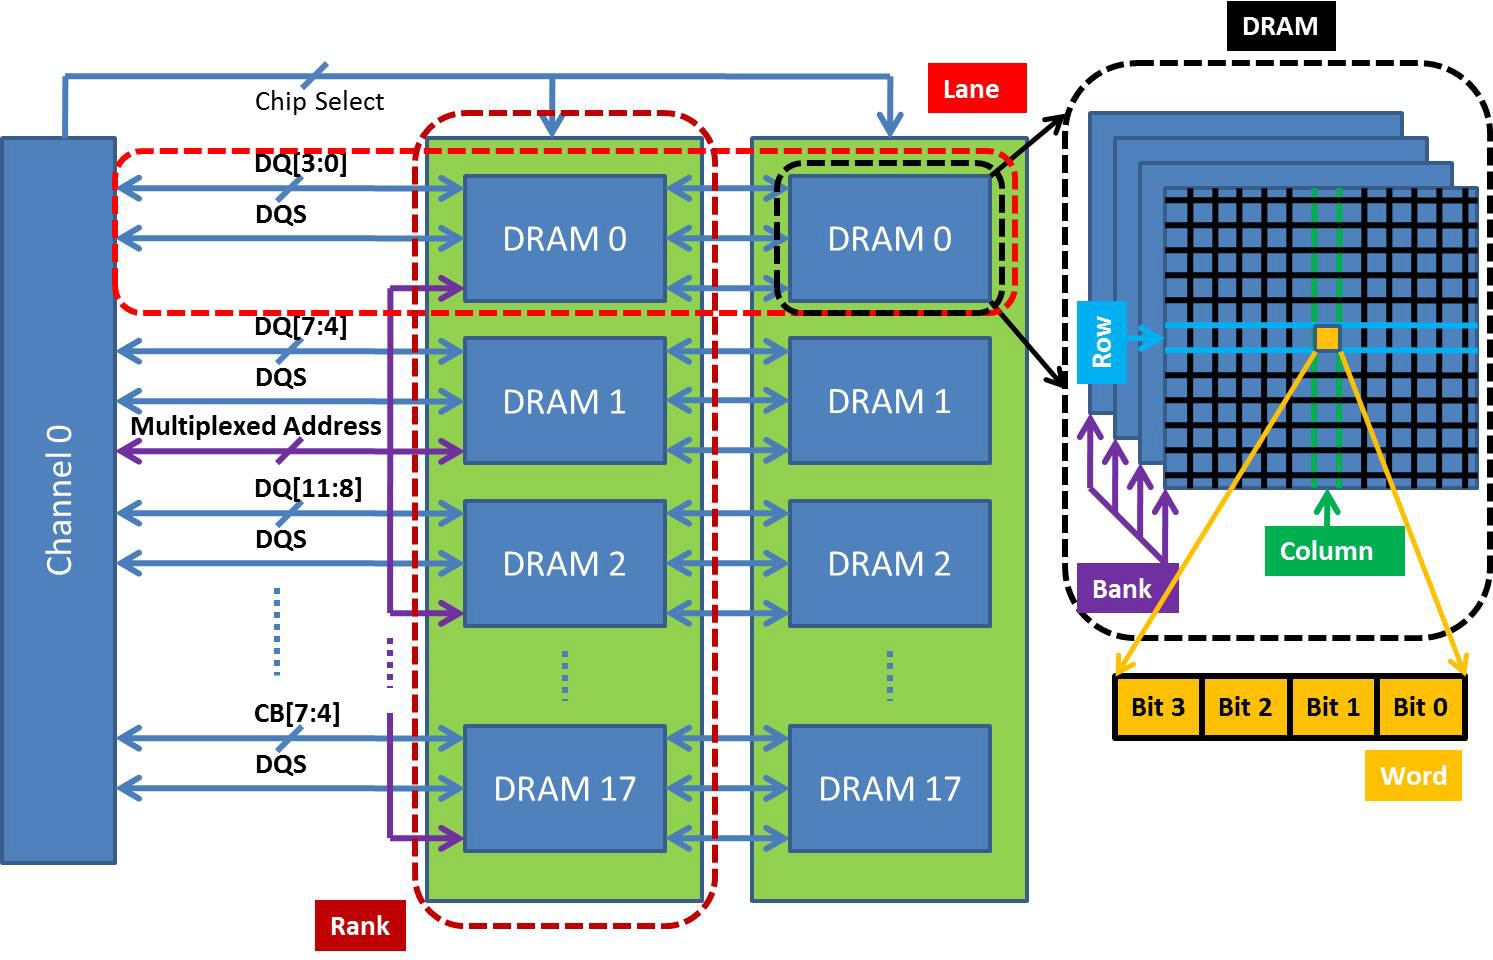
\includegraphics[width=5in]{exp.png}
    \caption{在Cielo和Hooper每个节点上DRAM内存的一个单通道的简化模型} \label{fig:exp}
  \end{center}
\end{figure}

作者进行分析时,使用了三种不同的数据集。分别是——来自控制台日志的纠正错误消息,事件日志的未校正错误消息和硬件清单日志。这三个日志提供了将每个错误消息映射到系统中存在于该时间点的特定硬件的能力。更正的错误日志包含特定时间戳的节点的事件。系统中的每个节点都有一个硬件存储控制器,用于在x86机器检查体系结构(MCA)提供的寄存器中记录更正的错误事件。

每个节点的操作系统都配置为每隔几秒轮询MCA寄存器,并将其发现的任何事件记录到节点的控制台日志中。未校正的错误事件日志类似,并包含系统中记录的未更正错误的数据。这些通常是不经过修正的错误导致的。控制台和事件日志都包含各种其他信息,包括与每个错误相关联的物理地址和ECC综合信息。

使用配置信息进一步解码这些事件以确定与每个错误相关联的物理DRAM位置。对于此分析,作者解码了显示DIMM的位置,以及DRAM库,列,行和芯片。作者假设每个DRAM器件在他们的观察间隔期间经历单个故障。每个DRAM故障的发生时间对应于每个DRAM器件首次观察到的错误消息的时间。然后,作者根据控制台日志中的相关错误为每个故障分配一个特定的类型和模式。

\subsection{故障模式}

作者确定了几种独特的DRAM故障模式:单位,其中所有错误映射到单个位; 单字,其中所有错误映射到单个字; 单列,其中所有错误映射到单个列; 单行,其中所有错误映射到单个行; 单组,其中所有错误都映射到单组; 多组,其中错误映射到多个组; 和多等级,其中错误映射到同一通道中的多个DRAM。


\subsection{实验结果选讲}

\subsubsection{高能粒子}
\begin{figure}[H]
  \begin{center}
    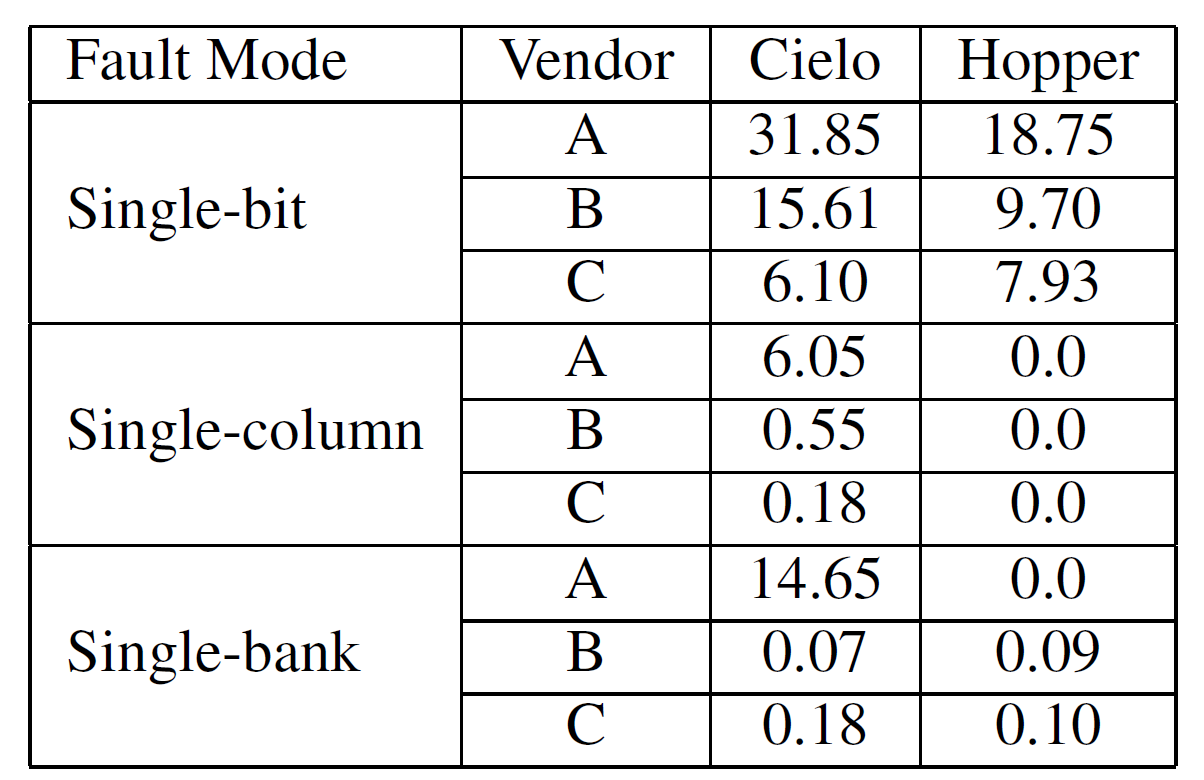
\includegraphics[width=5in]{single_bit_column_bank.png}
    \caption{单位、单列、单组故障率在Cielo和Hopper中的统计。Cielo中更高的瞬时错误可能说明这些故障是由高能粒子引发的。} \label{fig:single_bit_column_bank}
  \end{center}
\end{figure}

\subsubsection{海拔影响}
\begin{figure}[H]
  \begin{center}
    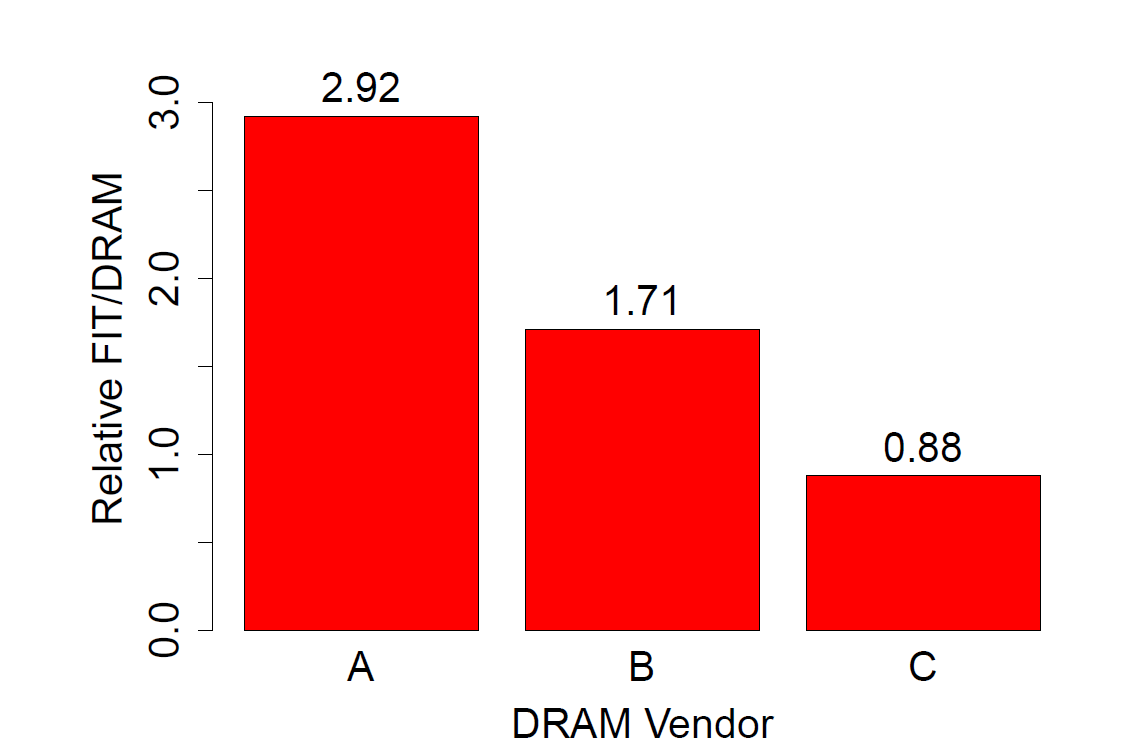
\includegraphics[width=5in]{dram_vendor.png}
    \caption{Cielo的DRAM瞬时故障率与Hopper的瞬时故障率相对大小(设Hopper=1.0)。供应商A显示了Cielo的瞬时故障率更高,很可能与海拔有关。} \label{fig:dram_vendor}
  \end{center}
\end{figure}

\subsection{实验结论}

\subsubsection{“好发现”}

\begin{itemize}
\item 现场大多数观察到的SRAM故障都是来自粒子撞击的瞬态故障。这进一步证实了SRAM故障是众所周知的现象和近期未来的工艺技术。
\item 大多数未校正的SRAM错误都是由于单位故障引起的; 因此,减少SRAM未校正的错误率是工程时间和精力的问题(例如,用ECC替换奇偶校验码),而不是新的研究和新技术。此外,适当的多位故障保护可降低或消除由于高空造成的SRAM故障导致的未校正错误率的预期增加。
\end{itemize}

\subsubsection{“坏发现”}
\begin{itemize}
\item 海拔提高了一些DRAM设备的故障率,虽然这种影响因供应商而异。这证明了一些(但不是全部)DRAM器件易受到高能量粒子撞击的瞬态故障的影响。
\item 与片上SRAM不同,未来系统的外部存储器(例如DRAM)将需要比现有超级计算系统中更强大的恢复技术。
\end{itemize}

\subsubsection{“丑发现”}
\begin{itemize}
\item 进行实地研究是困难的。例如,我们证明计数错误而不是故障可能导致关于系统可靠性的错误结论。我们检查最近使用错误计数的研究结果,并使用我们的数据来证明使用这种方法可能导致误导或不准确的结论。
\item SEC-DED ECC,一种常用的ECC技术,非常适合于现代DRAM子系统,并且可能导致未知的错误(可能导致无声数据损坏)到20FITperDRAM设备,这是许多企业数据中心和高性能计算系统的无法接受的高速率。
\end{itemize}

\section{不足之处与建议}

\subsection{对照实验的设置}

本文作者使用了两个在不同地点的顶尖的超级计算机来进行对比实验,来探究例如海拔对于内存故障率的影响。然而,在对照实验中,变量只能有一个——即要探究的变量。两个不同的超级计算机不仅有海拔不同,其所在地区的温度、湿度与供电情况甚至都不尽相同。

当然,理想的对照实验是不存在的。然而,仅仅用两个超算来探究不同变量对内存故障率的影响,我认为是不妥的。在条件允许的情况下,尽可能使用多的超算来探究不同变量的影响,我认为结果会更有说服力。

\subsection{干扰故障的确定}

6.1.2第二节:\emph{We did not do root-cause analysis on this part; therefore, we cannot say for certain that the fault in question is a disturbance fault. However, it is clear that fault modes with similar characteristics do occur in practice and must be accounted for.}

对于在该问题中的故障,作者并不确定是干扰故障。然而,可能由于进度或者技术的问题,并没有做进一步的研究,使得该问题十分模糊,没有得到完善的解答。

我认为,对于该问题,如果无法解决,至少应该写出自己做过的尝试。

\subsection{假设过于理想化}

8.1第二节:\emph{For the purposes of this study, we assume that errors larger than 2 bits in a single ECC word are undetectable by SEC-DED (an actual SEC-DED ECC typically can detect some fraction of these errors).}

作者做了SEC-DED ECC只能检测出两位及两位以下的单字错误的假设。然而在实际工作中,SEC-DED ECC可以检测出一些二位以上的单字错误。进行这样的假设,虽然便于研究,但是精确度会下降,结果的适用性会降低。

尽量减少与现实不符的假设,使用现实生活中的情况来进行研究。

\end{document}
